% =============================================================================
% CAPÍTULO 10 — volta 2, o teste da régua (AGENTS.md §6): a receita clássica de alerta
% precoce, submetida ao par que o capítulo do orçamento cobra de todo alarme.
%
% O fracasso que o abre, com número na mão: o limiar colhido como a prática colhe --- no
% desenho de um único mundo que muda --- gasta um alarme a cada 90,87 anos quando nada muda,
% sem que quem colheu soubesse, e chega 132 dias depois na rampa que o limiar calibrado
% anuncia em 84.
%
% Medição: lab/experimentos/E32_alerta.ipynb. Figuras: figuras/E32_alerta_*.
% =============================================================================

\chapter{O alerta que todo mundo usa}
\label{cap:alerta}

\section{O candidato que todo mundo usa}

O capítulo anterior instalou a régua --- medir um sinal exige medir o chão em que ele foi medido
--- e deixou na fila o candidato mais famoso de todos. Desde que os ecólogos notaram que lagos
turbam de uma vez e climas viram de regime, a prática vigia a mudança que ainda vem com uma
receita que tem nome e literatura: a janela curta do passado fica mais inquieta, os dias passam
a se parecer com os vizinhos, e esses números subindo antes da transição seriam o anúncio de
que ela vem\cite{scheffer2003catastrophic,scheffer2009early}. A receita virou método de
prateleira\cite{dakos2012methods}, atravessou da ecologia para os mercados e para o clima, e
chegou aos dados de hoje\cite{miramontes2026early}.

Só que a receita nunca declarou o par. Quanto ela soa quando nada muda, e quanto demora quando
algo muda --- as duas perguntas que o capítulo do orçamento transformou em obrigação de todo
alarme --- não estão nos papers; estão em nenhum lugar. Um indicador sem orçamento declarado
não é um alerta: é um desenho que sobe, com a esperança embaixo.

Este capítulo submete a receita à régua da casa, e o controle é o que a casa já tem: o
\textbf{posto do corte}, o dia que fica abaixo do pior dia dos últimos
\numAlertaJanela{} pregões --- o alarme mais fundo que a janela permite, irmão do vigia da
contagem. A pergunta é a da lista viva, no item que nomeia o adversário: os indicadores
clássicos de alerta precoce são a referência a bater, e este capítulo os mede no mesmo par em
que o posto já foi medido.

\section{O par que a receita nunca declarou}

A receita tem três pernas, e todas são estatísticas da mesma janela de
\numAlertaJanela{}\,dias que o livro usa desde o corte: a \textbf{variância} da janela, que
mede o tamanho dos dias; a \textbf{autocorrelação}, que mede a semelhança entre dias vizinhos;
e a \textbf{assimetria}, que mede de que lado os dias grandes caem --- a perna que falta para
a receita estar completa. Cada perna vira alarme por um limiar: a janela inteira acima da
linha, alarme.

% aterramento: assimetria

Duas decisões de medida, declaradas antes do número:

\begin{itemize}[leftmargin=1.5em]
  \item a unidade de gasto é o \textbf{episódio}, não o dia. A janela rolante arrasta o mesmo
    dia por dentro dela, e dias seguidos acima do limiar são um alarme só para quem ouve;
  \item o limiar de cada perna sai de uma bisseção em \numAlertaMundosParado{} mundos que
    nunca mudam, até gastar \textbf{exatamente o que o posto gasta, medido}:
    \numAlertaPostoEpisodiosAno{} episódios por ano. Orçamento igual para os quatro, medido e
    não prometido.
\end{itemize}

O resto é o mundo padrão da casa: \numAlertaCasos{} mundos novos por forma, mudança no meio
da série, horizonte de \numAlertaHorizonteDias{} dias para o alarme chegar. E há uma coluna
nova na tabela, que o capítulo anterior justificou: o \textbf{chão} de cada instrumento --- o
dia mediano do primeiro falso alarme em mundos que nunca mudam, contado do primeiro dia em que
o alarme existe. Latência menor que o chão é visão da mudança; latência do tamanho do chão é o
orçamento sendo gasto na frente dela.

\section{A medição: três formas e o chão}

\begin{table}[htbp]
  \centering
  \begin{tabular}{@{}lrrrr@{}}
    \hline
    instrumento & degrau & rampa & deriva & chão \\
    \hline
    posto & \numAlertaPostoDegrauDias & \numAlertaPostoRampaDias & \numAlertaPostoDerivaDias &
      \numAlertaPostoChaoDias \\
    variância & \numAlertaVarianciaDegrauDias & \numAlertaVarianciaRampaDias &
      \numAlertaVarianciaDerivaDias{} (\numAlertaVarianciaDerivaNadaPct\% não vê) &
      \numAlertaVarianciaChaoDias \\
    autocorrelação & \numAlertaAutocorrelacaoDegrauDias & \numAlertaAutocorrelacaoRampaDias &
      \numAlertaAutocorrelacaoDerivaDias{} (\numAlertaAutocorrelacaoDerivaNadaPct\% não vê) &
      \numAlertaAutocorrelacaoChaoDias \\
    assimetria & \numAlertaAssimetriaDegrauDias & \numAlertaAssimetriaRampaDias &
      \numAlertaAssimetriaDerivaDias{} (\numAlertaAssimetriaDerivaNadaPct\% não vê) &
      \numAlertaAssimetriaChaoDias \\
    \hline
  \end{tabular}
  \caption{Dias entre a mudança e o alarme: mediana de \numAlertaCasos{} mundos por forma,
    no mesmo orçamento de \numAlertaPostoEpisodiosAno{} episódios por ano. O chão é o primeiro
    falso alarme em mundo que nunca muda; na deriva, os mundos que não alarmaram até o
    horizonte de \numAlertaHorizonteDias{} dias vêm em porcentagem.}
  \label{tab:alerta_latencias}
\end{table}

\begin{figure}[htbp]
  \centering
  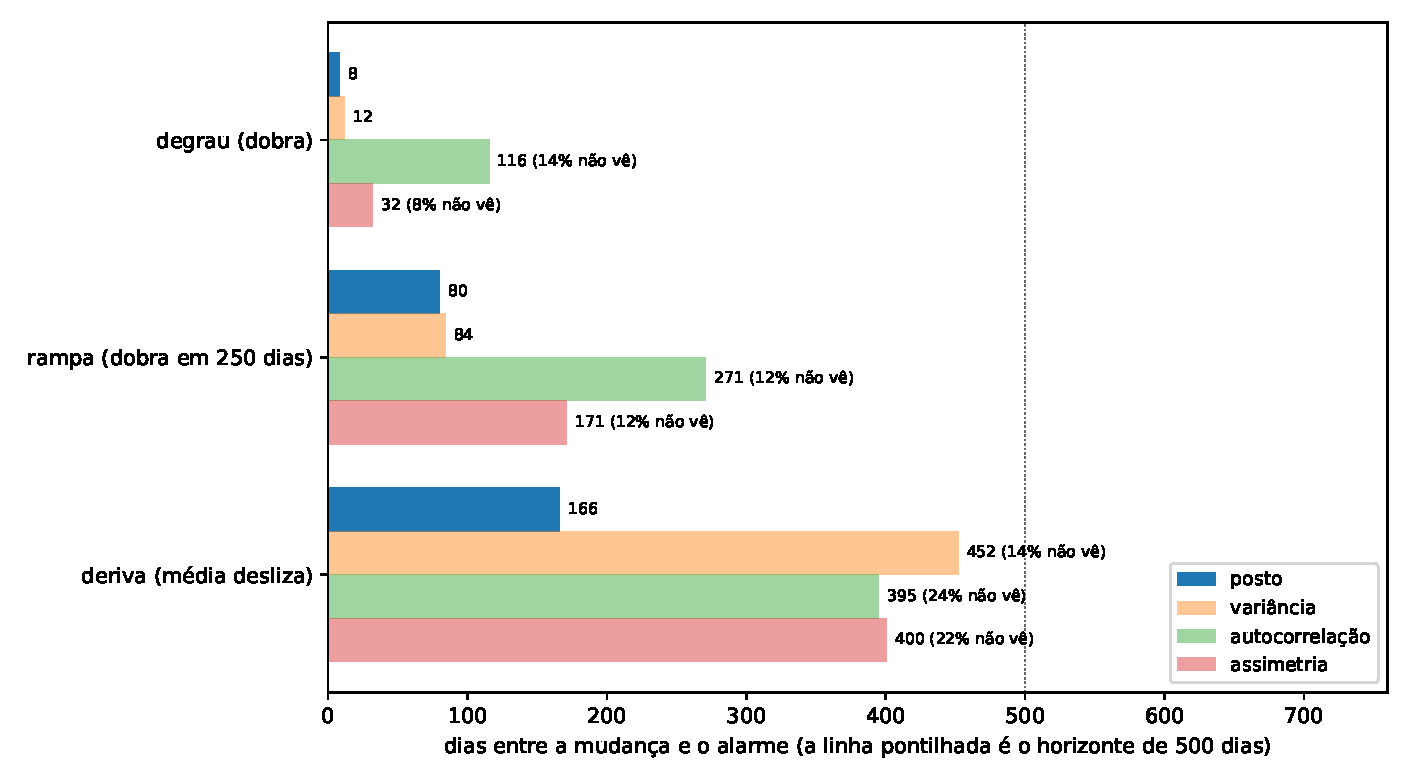
\includegraphics[width=\linewidth]{figuras/E32_alerta_1.pdf}
  \caption{A mesma tabela em barras: três grupos de forma, quatro instrumentos, o posto em
    azul cheio e as pernas da receita em meio-tom. A linha pontilhada é o horizonte de
    \numAlertaHorizonteDias{} dias. No degrau a barra do posto é a menor de todas; na rampa,
    posto e variância são quase a mesma barra; na deriva, as três barras da receita são as mais
    longas do desenho.}
  \label{fig:alerta_latencias}
\end{figure}

No \textbf{degrau}, o posto ganha de todos: \numAlertaPostoDegrauDias{} dias contra
\numAlertaVarianciaDegrauDias{} da variância, \numAlertaAssimetriaDegrauDias{} da assimetria e
\numAlertaAutocorrelacaoDegrauDias{} da autocorrelação --- e as duas últimas ainda deixam mundos
para trás. Que as pernas de ordem e de simetria atravessem o limiar no degrau não quer dizer
que o que elas medem tenha mudado: o dia que dobra de tamanho atravessa qualquer limiar que
esteja contando outra coisa.

Na \textbf{rampa}, o empate que decide o capítulo: \numAlertaPostoRampaDias{} dias do posto
contra \numAlertaVarianciaRampaDias{} da variância, os dois bem abaixo dos seus chãos --- os
dois veem a rampa de verdade, e nenhum vê melhor. É o terreno onde a receita nasceu, a
aproximação lenta da transição, e nele ela empata com o alarme mais fundo da janela.

Na \textbf{deriva}, ninguém: as quatro latências têm o tamanho dos seus chãos --- o posto em
\numAlertaPostoDerivaDias{} contra um chão de \numAlertaPostoChaoDias{}, a variância em
\numAlertaVarianciaDerivaDias{} contra \numAlertaVarianciaChaoDias{} ---, e as pernas da
receita ainda deixam de um septimo a um quarto dos mundos sem alarme nenhum. O capítulo da
forma já sabia: na deriva, quem enxerga é a média da janela, e nenhum alarme de rompimento.
A receita herdou a cegueira e não declarou.

E vale registrar a favor da casa: nos mundos novos, o posto repetiu a medição da volta do
orçamento --- degrau em dias, rampa em meses, deriva no chão --- dentro da variação de quem
sorteia mundos de novo. O instrumento da casa é o mesmo em qualquer sorteio.

\section{O limiar do olho}

Ninguém bissecciona limiar em duzentos mundos parados. A prática faz outra coisa: olha
\emph{um} mundo que muda, vê o indicador subir, e põe a linha onde o desenho parece alarmante.
O caderno fez exatamente isso --- a linha no meio da rampa de um único mundo sorteado --- e
mediu o que a linha compra.

O que ela compra é silêncio: em mundo que nunca muda, um alarme a cada
\numAlertaOlhoAnosPorAlarme{} anos --- \numAlertaOlhoEpisodiosAno{} episódios por ano, contra
os \numAlertaPostoEpisodiosAno{} do orçamento declarado. Quem colhe limiar no olho não escolhe
gastar pouco; escolhe sem saber o que está escolhendo. E paga na entrada: em rampas de mundos
que não foram olhados, o alarme demora \numAlertaOlhoRampaDias{} dias --- contra os
\numAlertaVarianciaRampaDias{} do limiar calibrado na mesma perna. A linha alta do olho é
tardia nas rampas baixas, e quem a colheu não tem o número que diria isso.

\section{Três mercados e dois tombos}

Os mundos sintéticos medem instrumentos; para ler mercado, o caderno calibrou de novo cada
perna em mundos parados gaussianos na escala de cada série --- \numAlertaMundosParado{} mundos
por série --- e contou episódios no índice americano S\&P 500, no Ibovespa e no % numeros-ok: nome próprio, não medição
Bitcoin, nos últimos vinte e cinco anos.

\begin{table}[htbp]
  \centering
  \begin{tabular}{lrrrr}
    \hline
    série & posto & variância & autocorrelação & assimetria \\
    \hline
    S\&P 500 & \numAlertaRealSpPostoEpisodiosAno & \numAlertaRealSpVarianciaEpisodiosAno & % numeros-ok: nome próprio
      \numAlertaRealSpAutocorrelacaoEpisodiosAno & \numAlertaRealSpAssimetriaEpisodiosAno \\
    Ibovespa & \numAlertaRealIbovPostoEpisodiosAno & \numAlertaRealIbovVarianciaEpisodiosAno &
      \numAlertaRealIbovAutocorrelacaoEpisodiosAno & \numAlertaRealIbovAssimetriaEpisodiosAno \\
    Bitcoin & \numAlertaRealBtcPostoEpisodiosAno & \numAlertaRealBtcVarianciaEpisodiosAno &
      \numAlertaRealBtcAutocorrelacaoEpisodiosAno & \numAlertaRealBtcAssimetriaEpisodiosAno \\
    \hline
  \end{tabular}
  \caption{Episódios por ano nas três séries, com limiares calibrados em mundos parados na
    escala de cada série. O declarado era \numAlertaPostoEpisodiosAno{} por ano; o posto entrega
    isso nas três, e as pernas da receita, não.}
  \label{tab:alerta_reais}
\end{table}

O posto entrega o que declarou nas três séries --- \numAlertaRealSpPostoEpisodiosAno{},
\numAlertaRealIbovPostoEpisodiosAno{} e \numAlertaRealBtcPostoEpisodiosAno{} episódios por ano
contra os \numAlertaPostoEpisodiosAno{} prometidos. A variância gasta um terço do declarado
(\numAlertaRealSpVarianciaEpisodiosAno{}, \numAlertaRealIbovVarianciaEpisodiosAno{},
\numAlertaRealBtcVarianciaEpisodiosAno{}): o limiar calibrado em mundos que oscilam todos os
dias fica alto para um mercado que oscila em pedaços. A assimetria inverte a história no
Ibovespa --- \numAlertaRealIbovAssimetriaEpisodiosAno{} por ano, acima do orçamento: o índice
tem assimetria de verdade, e a calibração gaussiana não contava com ela. Declarar o par não é
pedantismo contábil: é o que separa o alarme medido do alarme imaginado.

\begin{figure}[htbp]
  \centering
  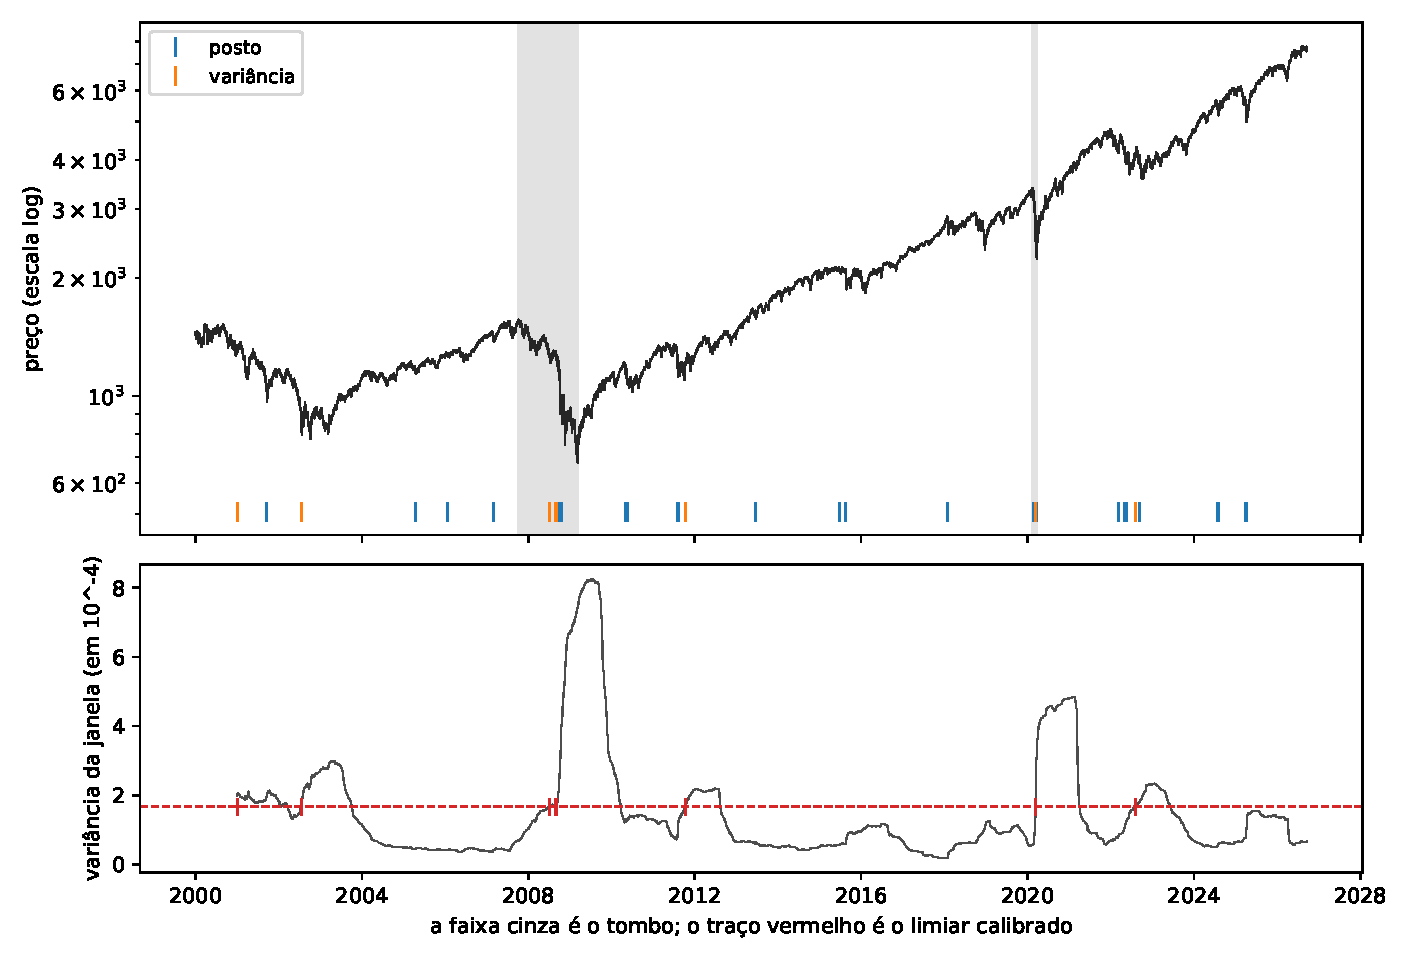
\includegraphics[width=\linewidth]{figuras/E32_alerta_2.pdf}
  \caption{O S\&P 500 em escala log com os dois tombos em faixa cinza, as marcas de alarme % numeros-ok: nome próprio
    na base --- o posto em azul, a variância em laranja --- e, embaixo, a variância da janela
    com o limiar calibrado em traço vermelho. Os dois instrumentos se acumulam nas mesmas % numeros-ok: nome próprio
    regiões de turbulência; na faixa de 2020, a marca do posto cai nos primeiros dias e a da % numeros-ok: nome próprio
    variância vem perto do fim da faixa.}
  \label{fig:alerta_real}
\end{figure}

Nos dois tombos do S\&P 500, a forma decidiu qual instrumento serviu. % numeros-ok: nome próprio

\begin{table}[htbp]
  \centering
  \begin{tabular}{lrr}
    \hline
    & dias após o topo & queda já paga \\
    \hline
    2008, posto & \numAlertaTomboAntigoPostoAtrasoDias & \numAlertaTomboAntigoPostoPagoPct\% \\ % numeros-ok: nome próprio
    2008, variância & \numAlertaTomboAntigoVarianciaAtrasoDias & % numeros-ok: nome próprio
      \numAlertaTomboAntigoVarianciaPagoPct\% \\
    2020, posto & \numAlertaTomboRecentePostoAtrasoDias & \numAlertaTomboRecentePostoPagoPct\% \\ % numeros-ok: nome próprio
    2020, variância & \numAlertaTomboRecenteVarianciaAtrasoDias & % numeros-ok: nome próprio
      \numAlertaTomboRecenteVarianciaPagoPct\% \\
    \hline
  \end{tabular}
  \caption{O alarme mais cedo de cada instrumento dentro de cada tombo, contado do topo. A
    queda já paga é a fração da queda total que tinha acontecido no dia do alarme.}
  \label{tab:alerta_tombos}
\end{table}

No tombo que moeu por um ano e meio --- o de 2008 ---, a variância soou primeiro: % numeros-ok: nome próprio
\numAlertaTomboAntigoVarianciaAtrasoDias{} dias após o topo, com
\numAlertaTomboAntigoVarianciaPagoPct\% da queda paga, contra
\numAlertaTomboAntigoPostoAtrasoDias{} dias e \numAlertaTomboAntigoPostoPagoPct\% do posto. No
tombo que veio de uma vez --- o de 2020 ---, a ordem trocou: o posto soou em % numeros-ok: nome próprio
\numAlertaTomboRecentePostoAtrasoDias{} dias com \numAlertaTomboRecentePostoPagoPct\% pago, e
a variância só em \numAlertaTomboRecenteVarianciaAtrasoDias{} dias, quando
\numAlertaTomboRecenteVarianciaPagoPct\% da queda já era passado. A janela longa da variância é
o que a fez ganhar o começo lento e perder o tombo rápido; o posto, que só olha para o pior dia
do último ano, fez o contrário. É a lição do capítulo da forma vista de dentro da receita ---
e é o registro honesto a favor dela: houve um tombo em que a receita ganhou.

\section{O que fica}

Fica o veredito, com o par na mesa: no mesmo orçamento declarado e medido, o alerta que todo
mundo usa não bateu o posto da casa. No degrau, perdeu de todos os lados; na rampa --- o
terreno onde nasceu ---, empatou; na deriva, foi tão cega quanto o resto, e sem declarar. As
pernas de ordem e de simetria atravessaram limiares sem que o que medem tivesse mudado, e o
limiar do olho comprou noventa anos de silêncio que ninguém escolheu. A referência a bater da
pergunta da lista foi medida, e está medida: o que falta na receita não é matemática, é o par.

Fica também a parte que a receita acertou, dita por inteiro: num tombo lento de mercado real,
a variância avisou dois meses antes do posto, e a um terço do prejuízo pago. A receita não é
inútil; é um instrumento sem termômetro --- funciona, e ninguém sabe em que régua.

E fica o fio para o capítulo seguinte. Receita e posto empataram na rampa bebendo da mesma
janela de \numAlertaJanela{}\,dias --- e o empate tem cheiro de teto: se os dois bebem da
mesma água, talvez não sejam dois. Quanto de pergunta cabe num pedaço finito de passado, e a
partir de quando explicações diferentes ficam indistinguíveis nele, é o que vem agora.
